\documentclass[aspectratio=169]{beamer}

% ---------- THEME & LOOK ----------
\usetheme{Madrid}
\usecolortheme{seahorse}
\usefonttheme{professionalfonts}
\setbeamertemplate{navigation symbols}{}
\setbeamercovered{transparent}
\setbeamertemplate{itemize items}[circle]
\setbeamertemplate{enumerate items}[default]
\setlength{\parskip}{0.25em}

% ---------- COLORS ----------
\usepackage{xcolor}
\definecolor{accent}{RGB}{0,92,184}
\setbeamercolor{structure}{fg=accent}
\setbeamercolor{title}{fg=white,bg=accent}
\setbeamercolor{frametitle}{fg=accent}
\setbeamercolor{block title}{bg=accent!10,fg=accent}
\setbeamercolor{block body}{bg=accent!3}

% ---------- PACKAGES ----------
\usepackage{booktabs}
\usepackage{amsmath, amssymb}
\usepackage{array}
\usepackage{hyperref}
\hypersetup{colorlinks=true,linkcolor=accent,urlcolor=accent}

% ---------- PLACEHOLDER BOX (compile-safe; no images required) ----------
\newcommand{\placeholderbox}[2][0.82\linewidth]{%
  \begin{center}
    \fbox{\begin{minipage}[c][0.46\textheight][c]{#1}
      \centering \vspace{0.25em}
      \textbf{#2}\\[0.6em]
      \emph{Insert figure/diagram here later.}
    \end{minipage}}
  \end{center}
}

% ---------- TITLE ----------
\title{\textbf{Labour Supply and Public Policy
 \vspace{.5cm}\\  }}
\subtitle{ {\large ECON 300 - Labour Economics}}
%\institute{UNBC}
\author{Muhebullah Karimzada}

\date{Winter 2026}

% ---------- SECTION INTRO SLIDES ----------
\AtBeginSection[]{
  \begin{frame}[plain]
    \transfade[duration=0.25]
    \centering
    {\usebeamerfont{title}\color{accent}\insertsectionhead}
    \vspace{0.8em}

    \begin{itemize}
      \item[] \textit{In this section we will:}
      \item<+-> Place each program into the income–leisure framework
      \item<+-> Compare work incentives via budget constraints
      \item<+-> Use diagrams (placeholders) you can fill later
    \end{itemize}
  \end{frame}
}

\begin{document}

% ============================================================
% TITLE
% ============================================================
\begin{frame}[plain]
  \titlepage
\end{frame}


\begin{frame}{Learning Objectives}
\transfade
\begin{itemize}
  \item Discuss key features of demogrants, social assistance, unemployment insurance, wage subsidies, workers’ compensation, and childcare subsidies.
  \item Use the labour supply model to analyze work incentives under demogrants, social assistance (with clawbacks), and wage subsidies.
  \item Analyze unemployment insurance within the income–leisure model and note empirical challenges.
  \item Graphically illustrate disability impacts on the budget constraint; compare compensation programs.
  \item Show how childcare costs and subsidies alter constraints and participation decisions.
\end{itemize}
\end{frame}

\begin{frame}{Main Questions}
\transfade
\begin{itemize}
  \item Can Canadian transfer programs be analyzed in a common framework to assess “best” designs for work incentives?
  \item Does unemployment insurance necessarily reduce incentives to work?
  \item Can welfare be designed to minimize adverse incentives while targeting need?
  \item How do we incorporate disabilities into the labour supply model and evaluate workers’ compensation?
  \item How do childcare costs and subsidies affect participation, hours, and the reservation wage?
\end{itemize}
\end{frame}


\begin{frame}{Income Maintenance Programs}
\transfade
\begin{itemize}
  \item Aim to supplement low incomes that arise for varied reasons; no single program fits all causes.
  \item Distinguish \textbf{permanent} (low wage) from \textbf{transitory} (hours shock) shortfalls—policy tools differ.
  \item \textbf{Universal} vs.\ \textbf{Targeted}: simplicity and coverage vs.\ cost and incentive effects.
\end{itemize}
\end{frame}

\begin{frame}{Universal vs.\ Targeted Programs}
\transfade
\begin{block}{Universal Programs}
Administratively simple; everyone receives the same transfer regardless of income. Expensive and benefits also flow to non-poor.
\end{block}
\begin{block}{Targeted Programs}
Cheaper: transfers top up to a threshold (e.g., poverty line) but can create \textbf{implicit taxes} on earnings that reduce work effort.
\end{block}
\end{frame}

\begin{frame}{TABLE 3.1: Government transfers received by Census Families in Canada, 2017}
\transfade
\small
\begin{tabular}{lcc}
\toprule
\textbf{Benefits} & \textbf{Percent of families} & \textbf{Average Amount} \\
\midrule
All government transfers (federal and provincial) & 83.7\% & \$12,750 \\
Federal Child Benefits & 20.2\% & \$6,314 \\
Provincial Child Benefits & 10.6\% & \$1,941 \\
Employment Insurance & 14.0\% & \$8,352 \\
Social Assistance & 11.3\% & \$8,367 \\
Workers’ Compensation & 3.5\% & \$9,820 \\
Canada/Quebec Pension Plan & 32.4\% & \$10,092 \\
Old Age Security & 25.1\% & \$8,566 \\
Guaranteed Income Supplement & 9.6\% & \$6,634 \\
\bottomrule
\end{tabular}
\end{frame}


\begin{frame}{Demogrants}
\transfade
\begin{itemize}
  \item Lump-sum transfer specific to a demographic group (e.g., OAS).
  \item \textbf{Work incentives:} No substitution effect; a pure \textbf{income effect} that tends to increase leisure and reduce hours.
  \end{itemize}
  \vspace{0.5cm}
\textbf{Note:} The income gain is partly “spent” on leisure, so income rises by less than the grant amount.

\end{frame}

\begin{frame}{Figure 3.1: Work Incentive Effects of a Lump-Sum Demogrant }
\centering
\vspace{2em}

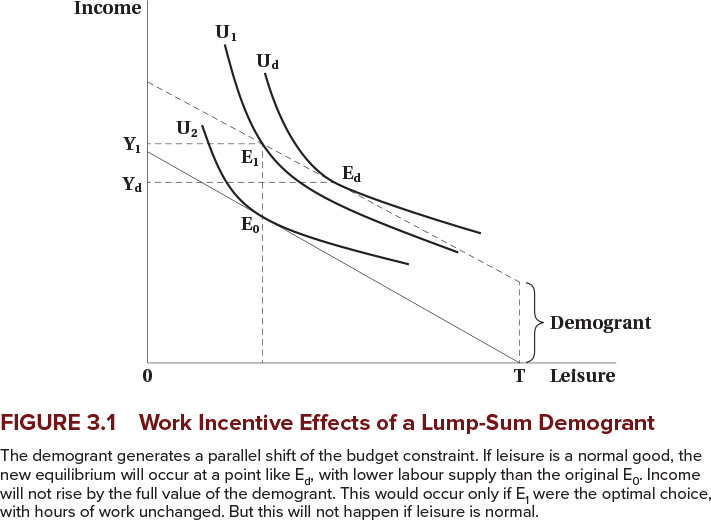
\includegraphics[width=0.77\linewidth]{ben54842_0301}.

\end{frame}

\begin{frame}{Welfare (Social Assistance)}
\transfade
\begin{itemize}
  \item Administered by provinces; partly financed by federal government.
  \item Benefits depend on need, assets, and other incomes.
\end{itemize}
\end{frame}

\begin{frame}{TABLE 3.2: Income of Welfare Recipients by Province, 2018 (lone parent, one child)}
\transfade
\small
\begin{tabular}{lcc}
\toprule
\textbf{Province} & \textbf{Annual Income\textsuperscript{a} (\$)} & \textbf{Income as \% of Poverty Line\textsuperscript{b}} \\
\midrule
Newfoundland & 23,436 & 85 \\
Prince Edward Island & 20,977 & 77 \\
Nova Scotia & 18,240 & 67 \\
New Brunswick & 19,978 & 78 \\
Quebec & 21,867 & 86 \\
Ontario & 21,463 & 72 \\
Manitoba & 21,764 & 82 \\
Saskatchewan & 21,087 & 77 \\
Alberta & 19,927 & 68 \\
British Columbia & 20,782 & 71 \\
\textbf{Average (unweighted)} & \textbf{20,952} & \textbf{76} \\
\bottomrule
\end{tabular}

\vspace{0.25em}
\scriptsize \textit{a.} Total annual income under program rules.\quad \textit{b.} Relative to poverty threshold used in the chapter.
\end{frame}

\begin{frame}{Figure 3.2: Work Incentive Effects of a Welfare Benefit with 100\% Clawback }
\centering
\vspace{2em}

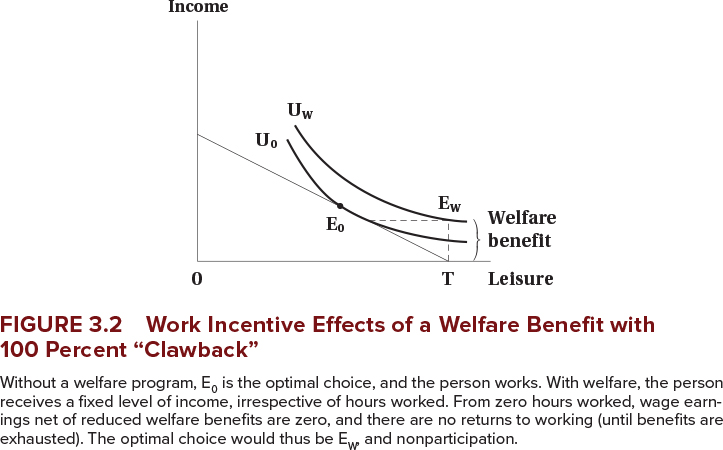
\includegraphics[width=0.98\linewidth]{ben54842_0302}.
\end{frame}

\begin{frame}{Improving Work Incentives in Welfare}
\transfade
\begin{itemize}
  \item Reduce the welfare benefit level (lower income effect).
  \item Raise the wage rate (tilt budget upward).
  \item Reduce the implicit tax rate (partial clawback).
  \item Shift preferences (e.g., work supports) toward market work.
\end{itemize}
\end{frame}

\begin{frame}{Figure 3.3: Other Work Incentive Effects of Welfare Programs }
\centering
\vspace{2em}

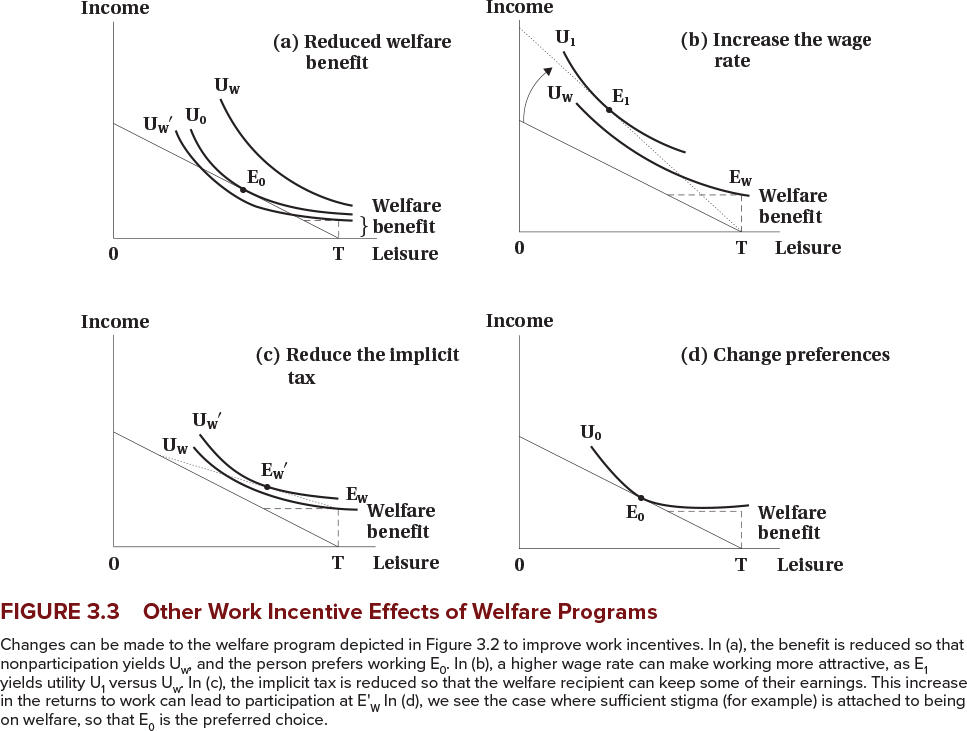
\includegraphics[width=0.72\linewidth]{ben54842_0303}.
\end{frame}

\begin{frame}{Figure 3.4: Welfare Benefits, Beneficiaries, and Labour Market Conditions (Ontario)}
\centering
\vspace{2em}

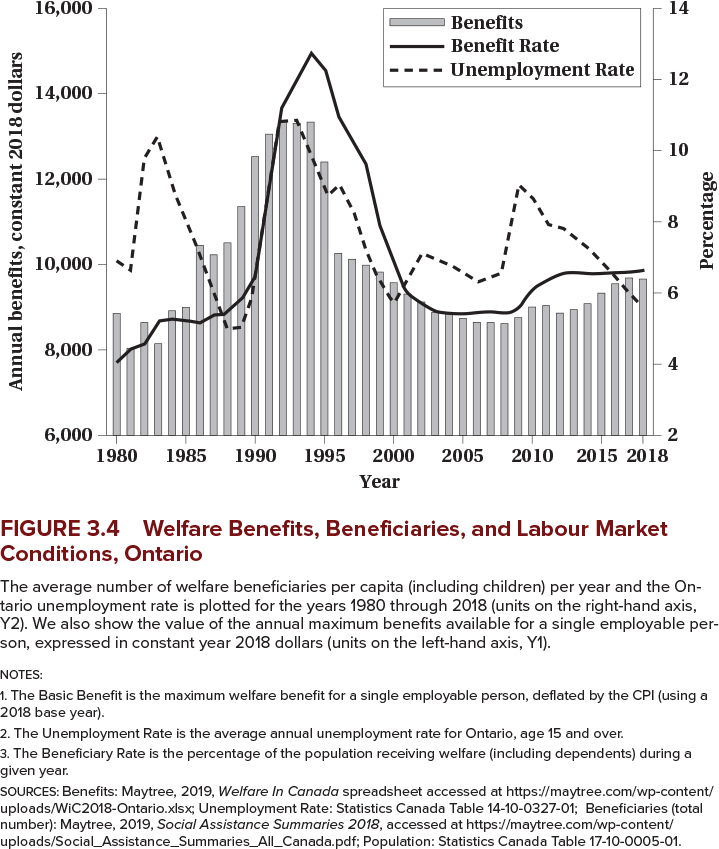
\includegraphics[width=0.62\linewidth]{ben54842_0304}.
\end{frame}

\begin{frame}{Negative Income Tax (NIT)}
\transfade
\small
\textbf{Income guarantee with partial clawback:}
\[
Y = G + (1 - t)E
\]
\begin{itemize}
  \item \(G\): guaranteed income;\; \(t\): implicit tax rate;\; \(E\): earnings.
  \item Reduces hours via income effect and partial substitution effect (slope changes).
  \item Can replace welfare schemes with harsher disincentives.
\end{itemize}
\end{frame}

\begin{frame}{Figure 3.5: Work Incentive Effects of a Negative Income Tax }
\centering
\vspace{2em}

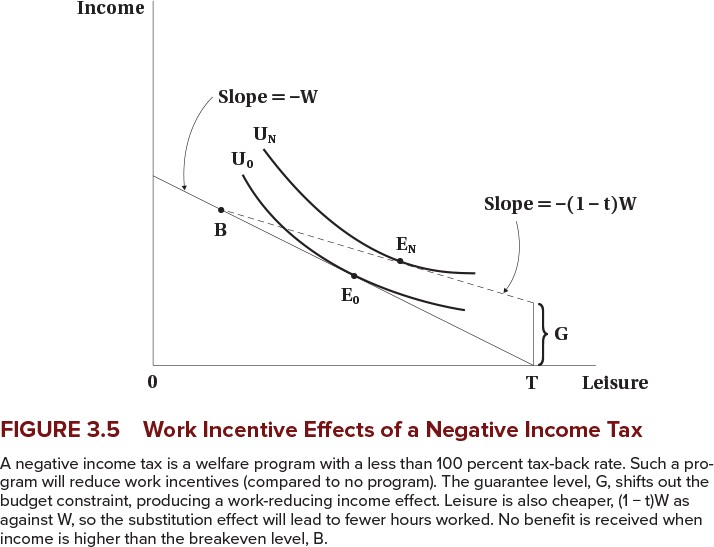
\includegraphics[width=0.76\linewidth]{ben54842_0305}.
\end{frame}

\begin{frame}{Wage Subsidy}
\transfade
\begin{itemize}
  \item Subsidizes earnings; raises effective wage.
  \item \textbf{Theoretical net effect on hours is indeterminate} (income vs.\ substitution work in opposite directions).
  \item Less adverse than a pure NIT for workers but does not help those unable to work.
\end{itemize}
\end{frame}

\begin{frame}{Figure 3.6: Work Incentive Effects of a Wage Subsidy }
\centering
\vspace{2em}

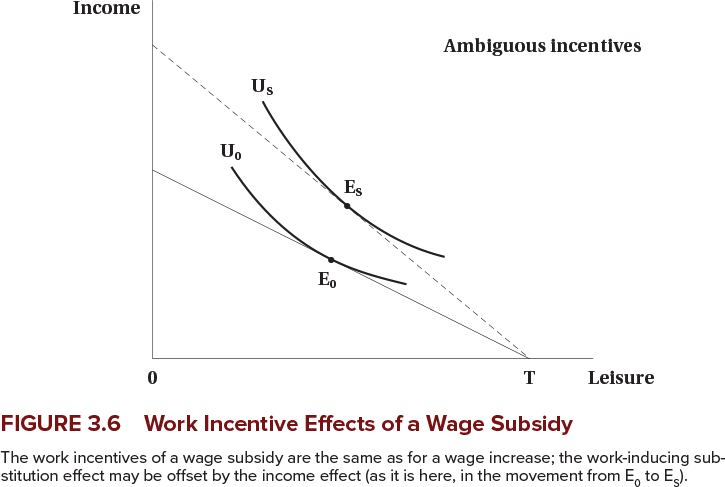
\includegraphics[width=0.82\linewidth]{ben54842_0306}.
\end{frame}

\begin{frame}{Refundable Tax Credit (Targeted Wage Subsidy)}
\transfade
\begin{itemize}
  \item Income-tested wage subsidy: \textbf{phase-in}, \textbf{flat}, and \textbf{phase-out} regions.
  \item Phase-in: substitution \(\uparrow\) (work more) vs.\ income \(\uparrow\) (work less) \(\Rightarrow\) ambiguous net.
  \item Flat: income effect only \(\Rightarrow\) hours fall (if leisure is normal).
  \item Phase-out: acts like NIT; substitution and income effects reduce work; participation effects can be clearer than hours.
\end{itemize}
\end{frame}

\begin{frame}{Figure 3.7: Work Incentives of a Refundable Tax Credit}
\centering
\vspace{2em}

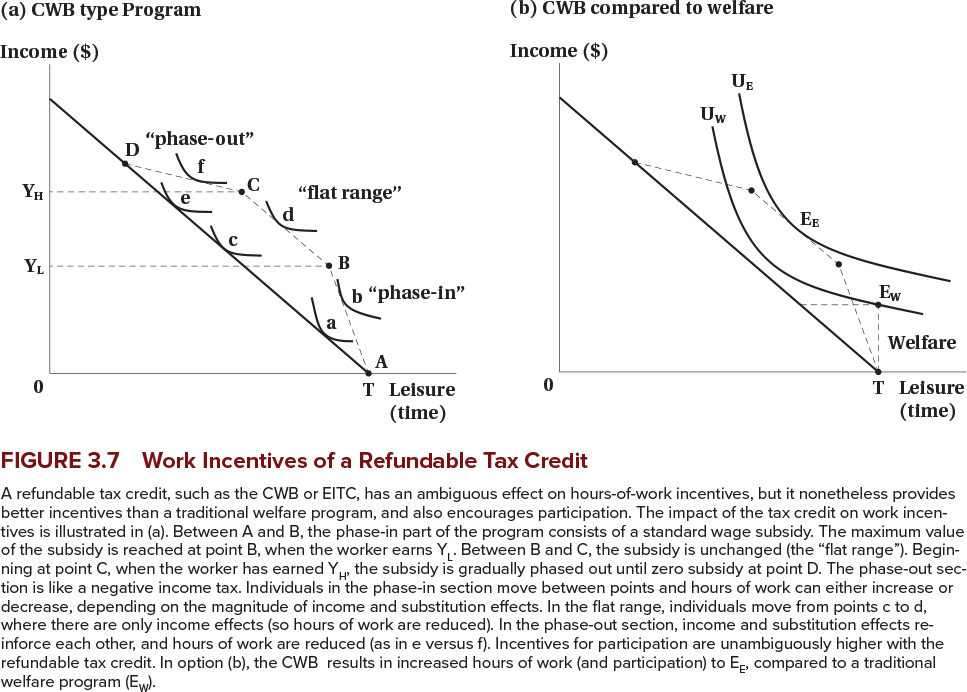
\includegraphics[width=0.955\linewidth]{ben54842_0307}.
\end{frame}


\begin{frame}{Unemployment Insurance (EI): Key Features}
\transfade
\begin{itemize}
\item Canada's unemployment insurance program, known as Employment Insurance EI since 1996, is the largest income security program for non-elderly individuals in the country
\item[]
\item The amount of income replacement rate is $55\%$ of lost earning, subject to a maximum
\item[]
\item The duration of benefit ranges from 14 to 45 weeks, depending on the regional rate of unemployment
\item[]
 \item In order to qualify for the benefits, individuals must have worked between 420 and 700 hours, the equivalent of 12-20 weeks at 35 hours per week, again depending on the unemployment rate of the region.
\end{itemize}
\end{frame}

















\begin{frame}{Worked Example: Unemployment Insurance and Work Incentives}
\transfade
\small
Example\\

Analysing the work incentive effects of unemployment insurance using the income-leisure model of the labour supply 

\begin{itemize}
\item[]
\item Recipients receive 60 percent of their weekly pay in the case of unemployment 

\item[]
\item It requires a minimum of 14 weeks of employment in order to qualify for benefits.

\item[]
\item The maximum period of receiving benefits is 20 weeks
\item[]
\item For simplicity,  we use one-year time horizon
\end{itemize}
\end{frame}

\begin{frame}{Income Constraint for a Simplified Unemployment Insurance Scheme }
\centering
\vspace{2em}

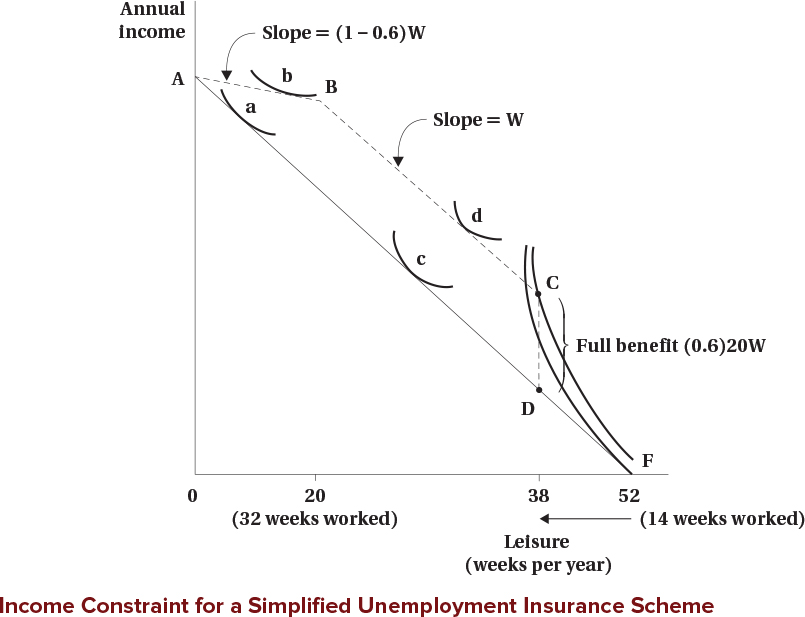
\includegraphics[width=0.61\linewidth]{ben54842_un0301}.
\end{frame}


 \begin{frame} \frametitle{Income Constraint for a Simplified Unemployment Insurance Scheme}
\transfade

\begin{itemize}
\item[]
\item AF (solid line)- potential income constraint in the absence of unemployment insurance (UI) program

\item[]
\item ABCDF- constraint with UI

\item[]
\item If the individual works less than 14 weeks during the year,  they do not qualify for UI benefits - their income constraint is segment DF
\item[]
\item If the individual works 14 weeks,  they are eligible for benefits for an additional 20 weeks
\item[]
\item Their income at 14 weeks of work equals their labour market earning for the 14 weeks plus 20 times 60 percent of their normal weekly wage earnings
\item[]
\item Their annual income would be $Y=14W +(0.60)20W$
 \end{itemize}
 \end{frame}


 \begin{frame} \frametitle{Income Constraint for a Simplified Unemployment Insurance Scheme}
\transfade

\begin{itemize}
\item[]
\item Their annual income would be $Y=14W +(0.60)20W$
\begin{itemize}
\item W is weekly wage earnings
\item $(0.60)20W$ - full benefit (vertical distance between C and D)
\item[]
\end{itemize}
 \end{itemize}

The work incentive effects of UI depend on where the individual would be located in the absence of UI system - three different possibilities

\begin{enumerate}
\item Individuals working more than 32 weeks (e.g. point a on AF)

\begin{itemize}
\item The income and substitution effects work in the same direction to potentially decrease weeks worked (moving to point b on AB)
\end{itemize}

\item Individuals such as those originally at point c on AF
\begin{itemize}
\item the UI system constitutes pure income effect - potentially decreasing work incentives (moving to point d on AB)
\end{itemize}
\end{enumerate}
 \end{frame}
 
 
  \begin{frame} \frametitle{Income Constraint for a Simplified Unemployment Insurance Scheme}




\begin{enumerate}
\setcounter{enumi}{2}
\item Individuals who would be outside the labour force in the absence of UI program
\begin{itemize}
\item[]
\item originally locted at point F -  reflecting the high value of their time devoted to non-market activities
\item[]
\item many of these individuals neither work nor collect UI
\item[]
\item others would enter the labour force and work a sufficient number of weeks to qualify for UI benefits (point C)
\begin{itemize}
\item[]
\item UI program has increased work incentives by making it attractive for these individuals to devote less time to non-market activities and to enter the labour force for relatively brief periods.
\end{itemize}
\end{itemize}
\end{enumerate}
 \end{frame}

\begin{frame}{Effect of a Disability}
\transfade
\begin{itemize}
  \item Alters budget (medical costs, fewer feasible hours) and/or preferences (higher disutility of work).
  \item Consider hours able to work, medical expenses, reduced wage-earning capacity, and relative disutility of market work.
\end{itemize}
\end{frame}

\begin{frame}{Figure 3.8: Effect of Disability }
\centering
\vspace{2em}

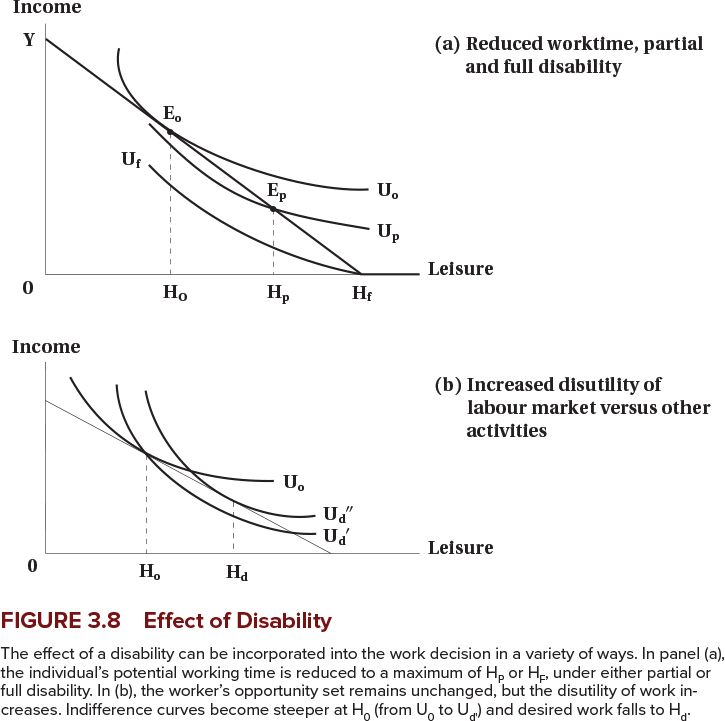
\includegraphics[width=0.55\linewidth]{ben54842_0308}.

\end{frame}




 \begin{frame} \frametitle{Child Care Benefit}
\label{Child Care Benefit}

\begin{itemize}
\item Analysis of the child care benefit first requires an investigation of how child care costs might affect a parent's labour supply decision

\item Child care costs can be modelled as a special case of fixed costs associated with working

\item Assumptions:
\begin{itemize}


 \item child care cost is incurred only if the person works in paid labour market
\item child care cost is independent of hours worked
\item[]
\end{itemize}

 \end{itemize}
 \end{frame}
 
 
  \begin{frame}
  \frametitle{The effect of Child Care Costs on Labour Supply
}
\begin{figure}
    \begin{center}
      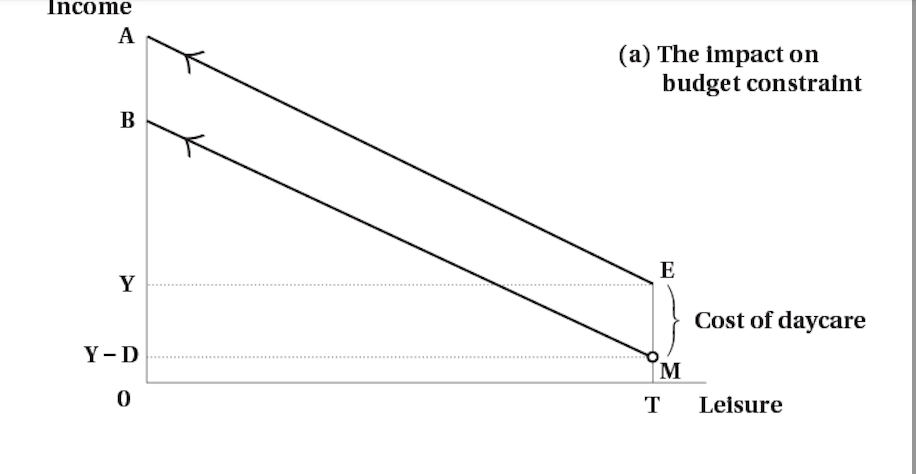
\includegraphics[scale=0.76]{CCB1.png}
      %    \includegraphics[scale=.40]{one.pdf}
      \end{center}
  \end{figure}
\end{frame}
 
 
   \begin{frame}
  \frametitle{The effect of Child Care Costs on Labour Supply}
The impact on budget constraint:

\begin{itemize}

\item the fixed cost of child care is analogous to a vertical drop in the individual's budget constraint immediately upon entering the labour market
\begin{itemize}
\item[]
\item the individual incurs the fixed costs D=EM $\rightarrow$ analogous to a drop in income of EM
\item[]
\item point M is slightly to the left of the vertical line ET - indicating that costs are incurred only if one engages in labour market activity
\item[]
\item fixed costs are avoided if one does not work in the labour market but remains at E

\end{itemize}
\end{itemize}
Summary:
\begin{itemize}
\item Income constraint AE - in the absence of child care costs
\item Income constraint BME - with fixed child care costs
\end{itemize}
\end{frame}
 
 
 %   \begin{frame}
 % \frametitle{The effect of Child Care Costs on Labour Supply
%}
%\begin{figure}
  %  \begin{center}
   %   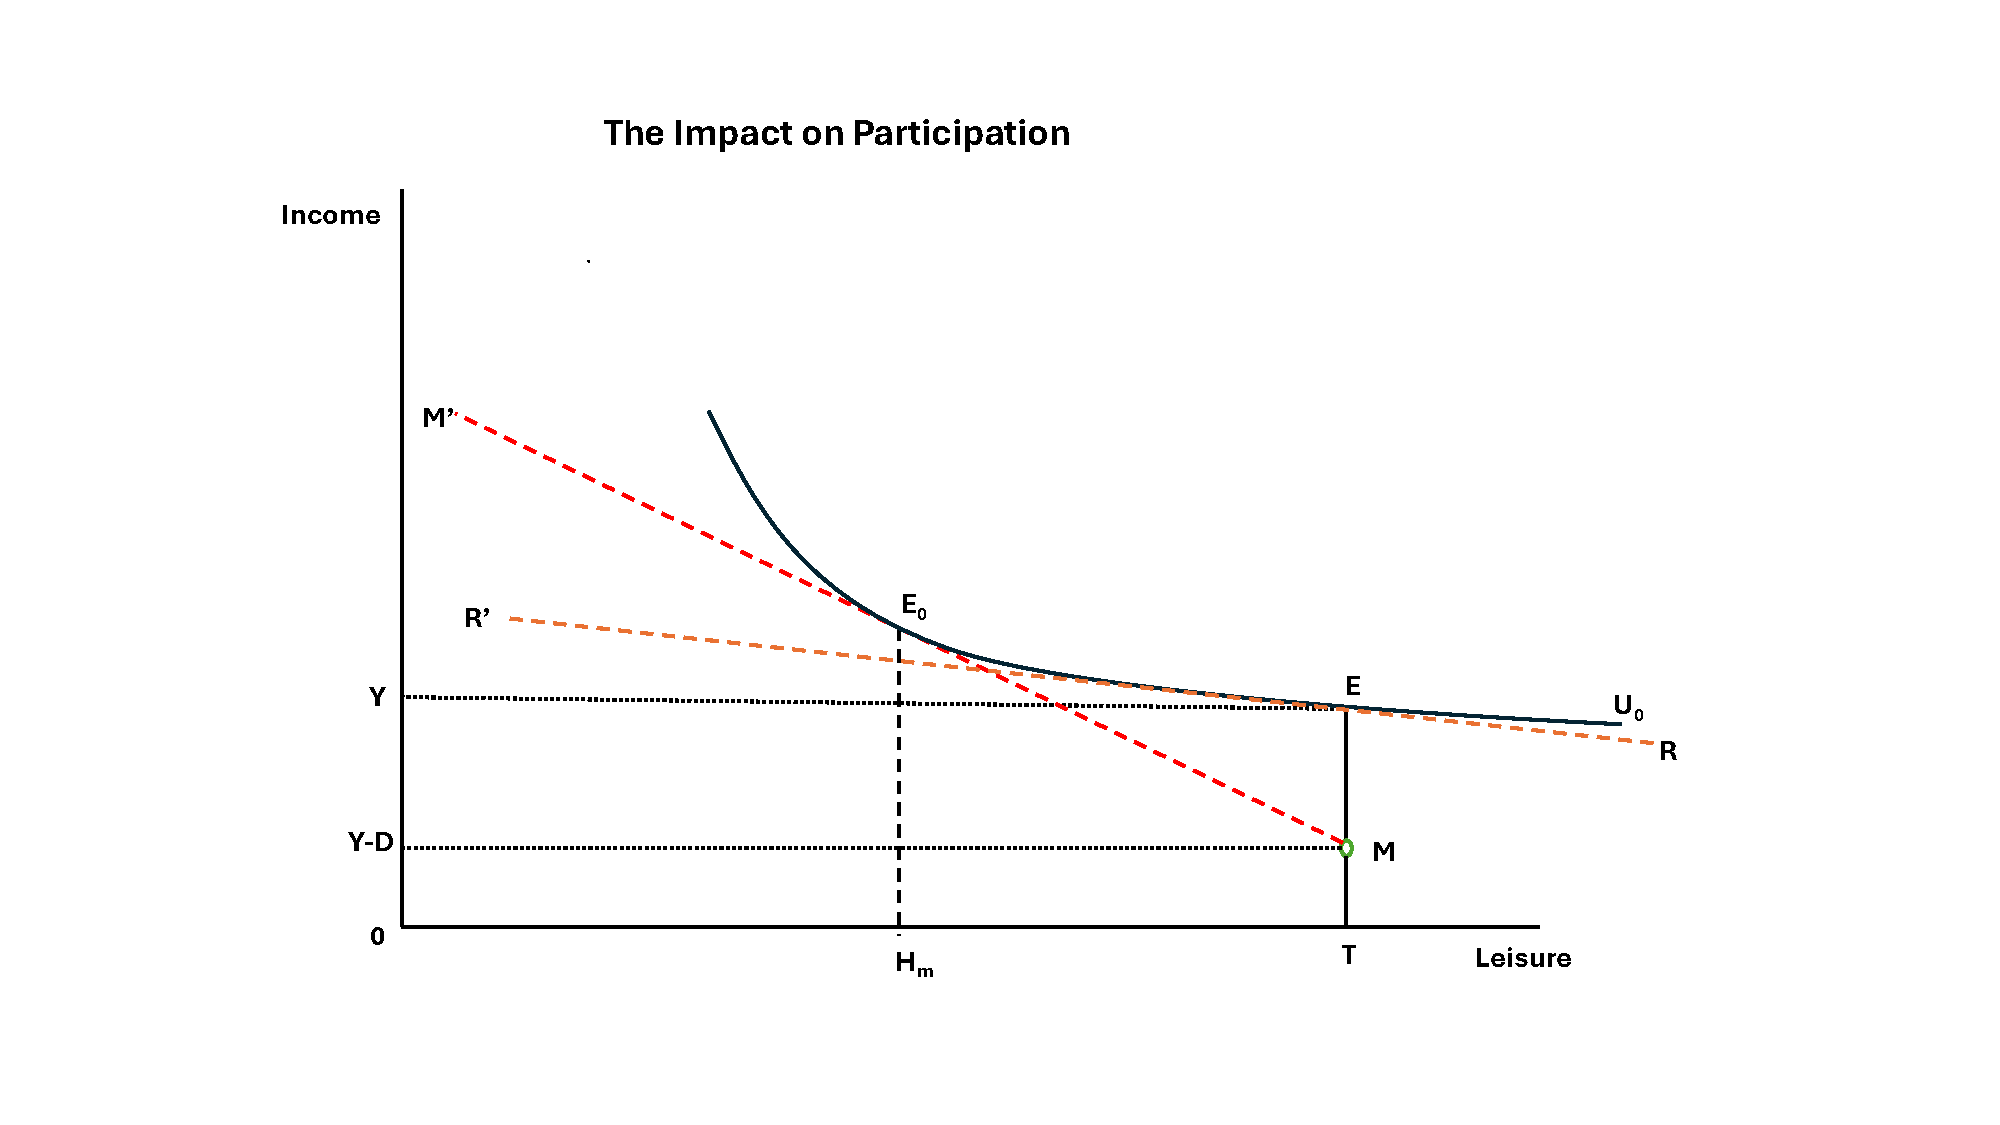
\includegraphics[scale=0.4]{Presentation1b.pdf}
      %    \includegraphics[scale=.40]{one.pdf}
   %   \end{center}
 % \end{figure}
%\end{frame}

   \begin{frame}
  \frametitle{The effect of Child Care Costs on Labour Supply
}
\begin{figure}
    \begin{center}
      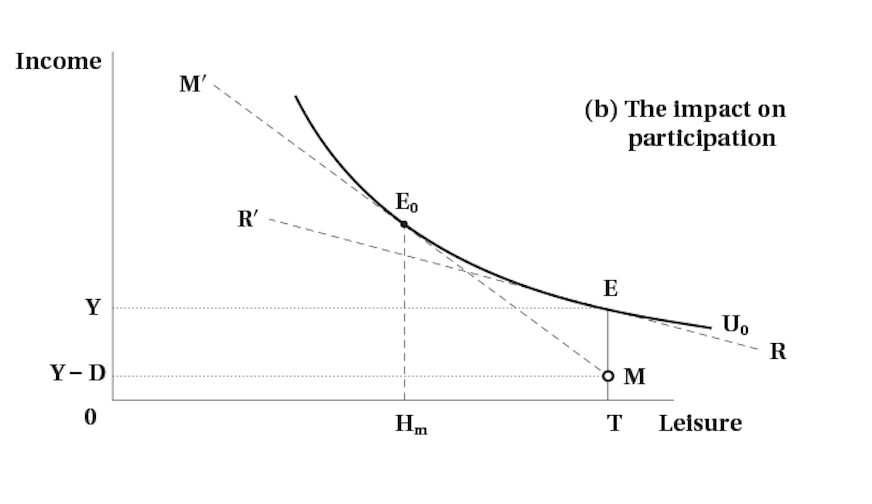
\includegraphics[scale=0.76]{CCB2.png}
      %    \includegraphics[scale=.40]{one.pdf}
      \end{center}
  \end{figure}
\end{frame}
 
 
   \begin{frame}
  \frametitle{The effect of Child Care Costs on Labour Supply}
The impact on participation:

\begin{itemize}
\item In the absence of child care fixed costs, the individual's reservation wage is depicted by the slope RR'
\item[]
\item In the presence of child care fixed costs, the individual's reservation wage is depicted by the slope MM'
\begin{itemize}
\item[]
\item the minimum wage above which one would enter the labour market
\item[]
\item at this wage one would be indifferent between engaging in labour market activities at $E_{0}$ and remaining at home with children at E
\item[]
\end{itemize}

\item Market wage greater than the reservation wage would induce labour force participation and the amount of work would be determined by the tangency of new, higher indifference curve and a higher budget constraint

\end{itemize}

\end{frame} 
 
 
    \begin{frame}
  \frametitle{The effect of Child Care Costs on Labour Supply}
The impact on participation:

\begin{itemize}

\item the line MM' is tangent to $U_{0}$ at the point  $E_{0}$ that is to the left of E of the same indifference curve
\item[]
\item the indifference curve become steeper as one moves to the left of E because of the hypothesis of diminishing marginal rate of substitution
\item[]
\item child care costs associated with entering the labour market increase the reservation wage by making labour market work less attractive than caring for the children at home

\end{itemize}

\end{frame} 
 
 
    \begin{frame}
  \frametitle{The effect of Child Care Costs on Labour Supply
}
\begin{figure}
    \begin{center}
      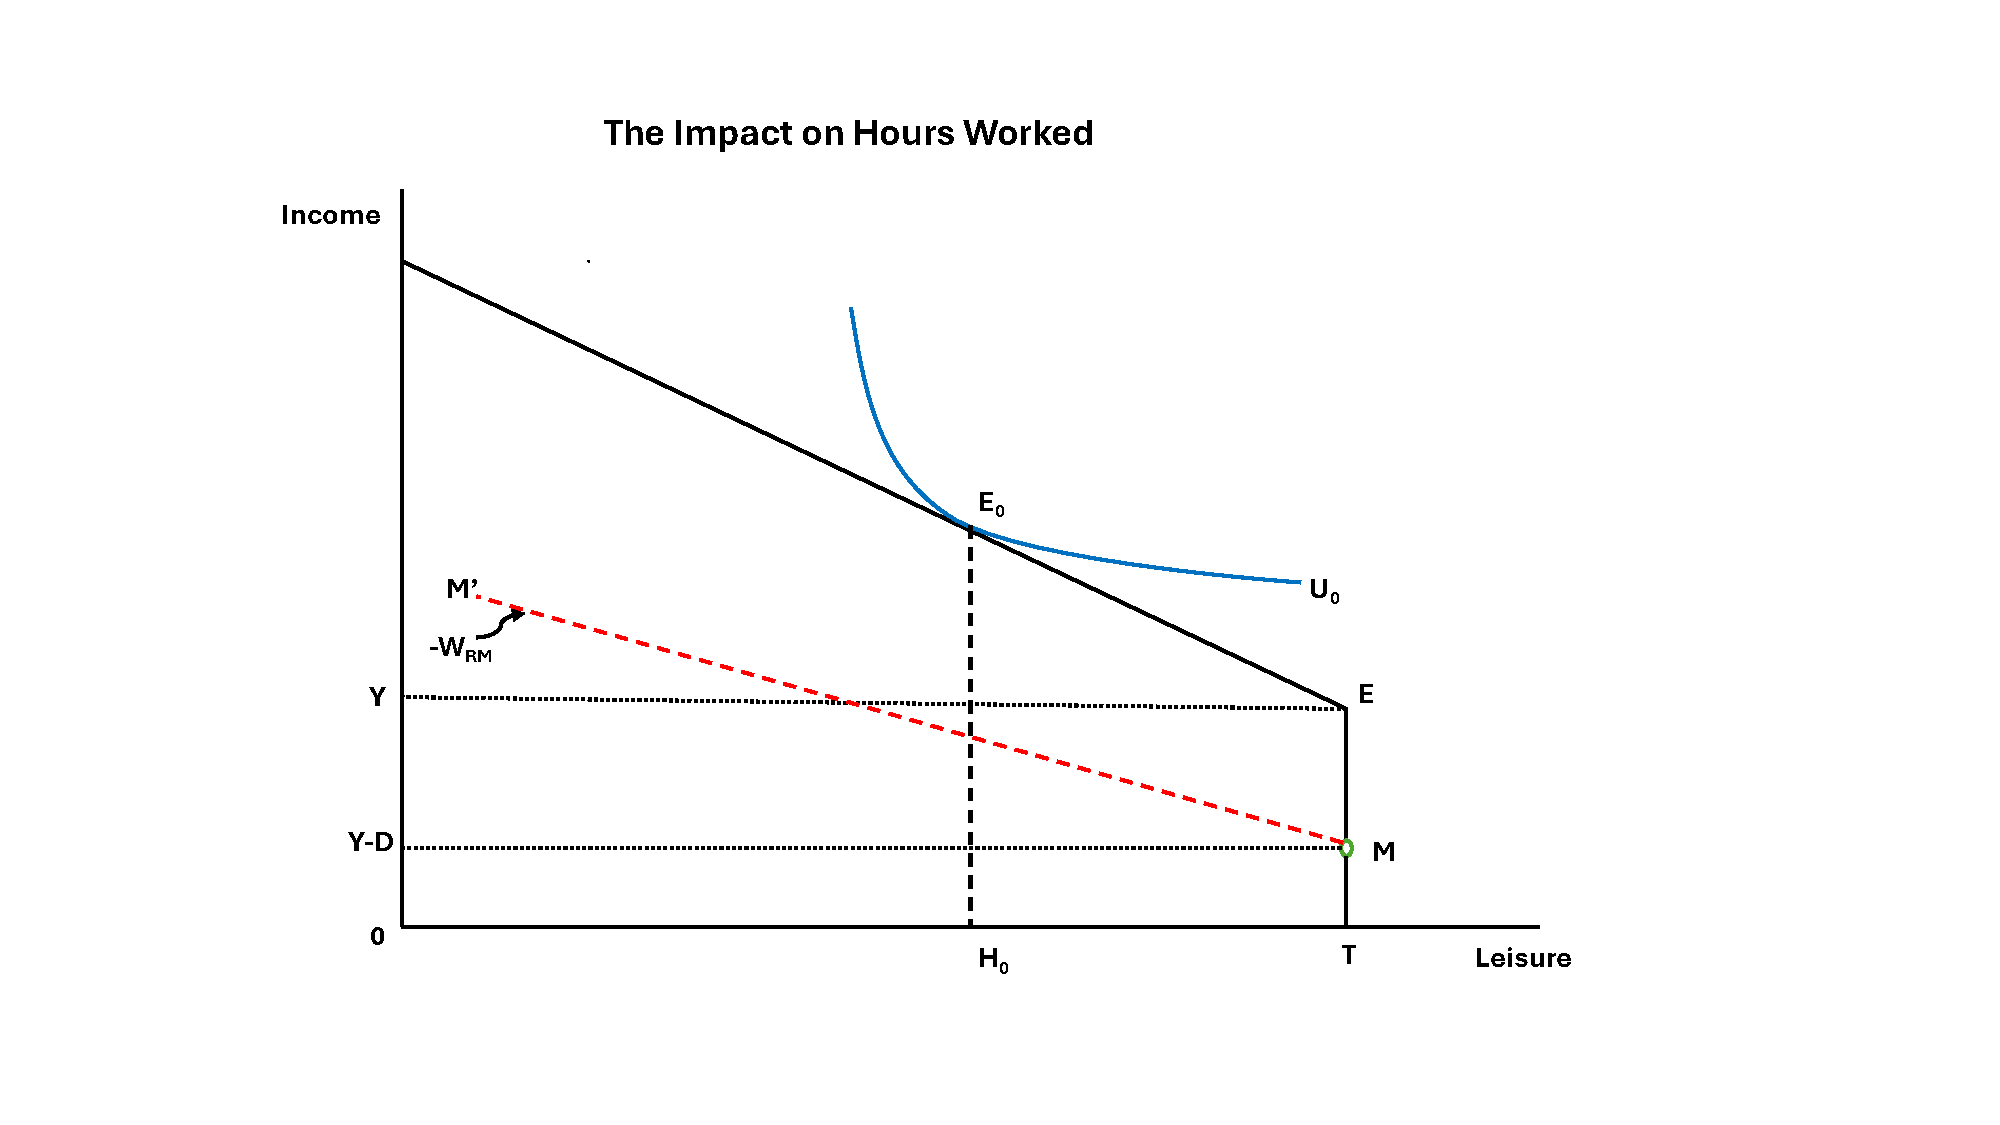
\includegraphics[scale=0.43]{Presentation2.pdf}
      %    \includegraphics[scale=.40]{one.pdf}
      \end{center}
  \end{figure}
\end{frame}
 
    \begin{frame}
  \frametitle{The effect of Child Care Costs on Labour Supply
}
\begin{figure}
    \begin{center}
      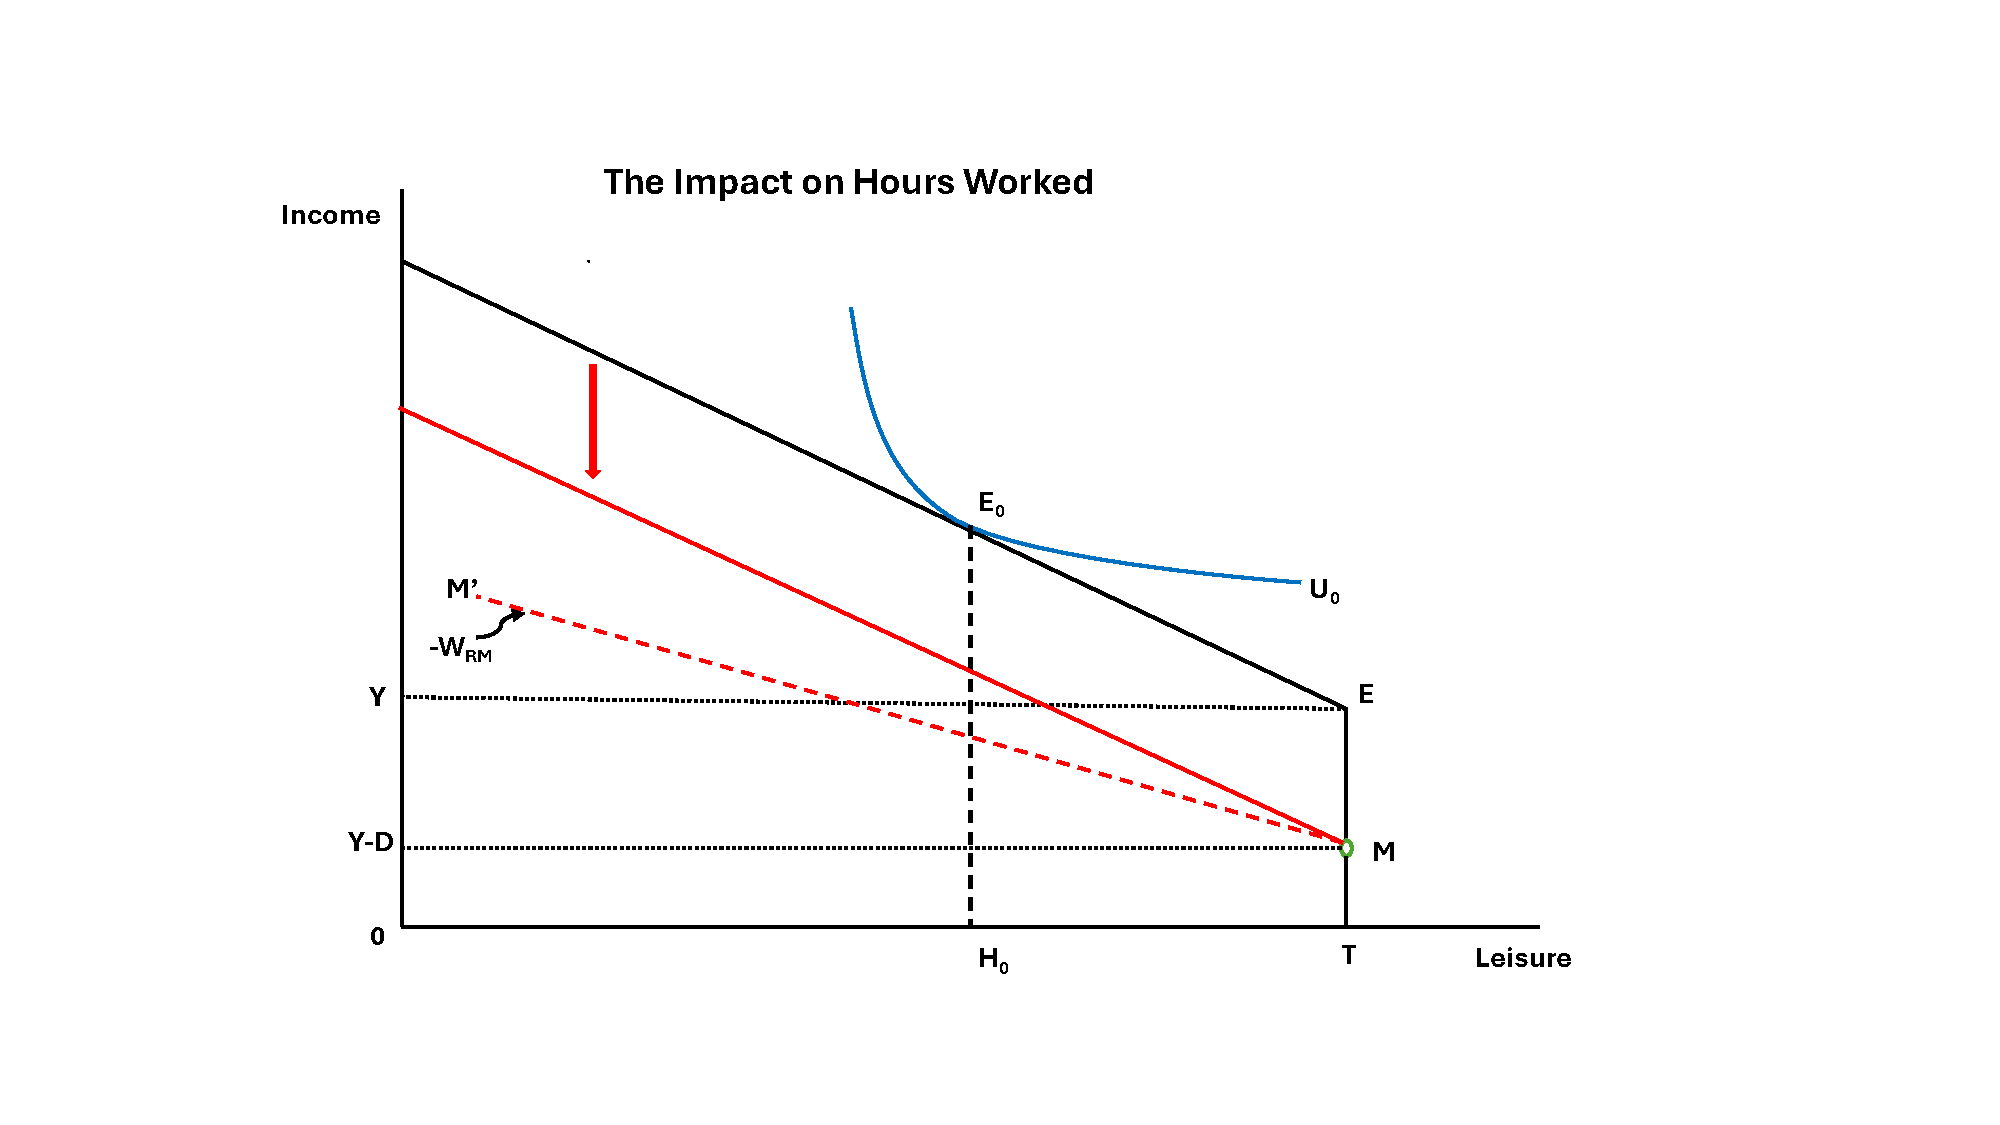
\includegraphics[scale=0.43]{Presentation3.pdf}
      %    \includegraphics[scale=.40]{one.pdf}
      \end{center}
  \end{figure}
\end{frame}

    \begin{frame}
  \frametitle{The effect of Child Care Costs on Labour Supply
}
\begin{figure}
    \begin{center}
      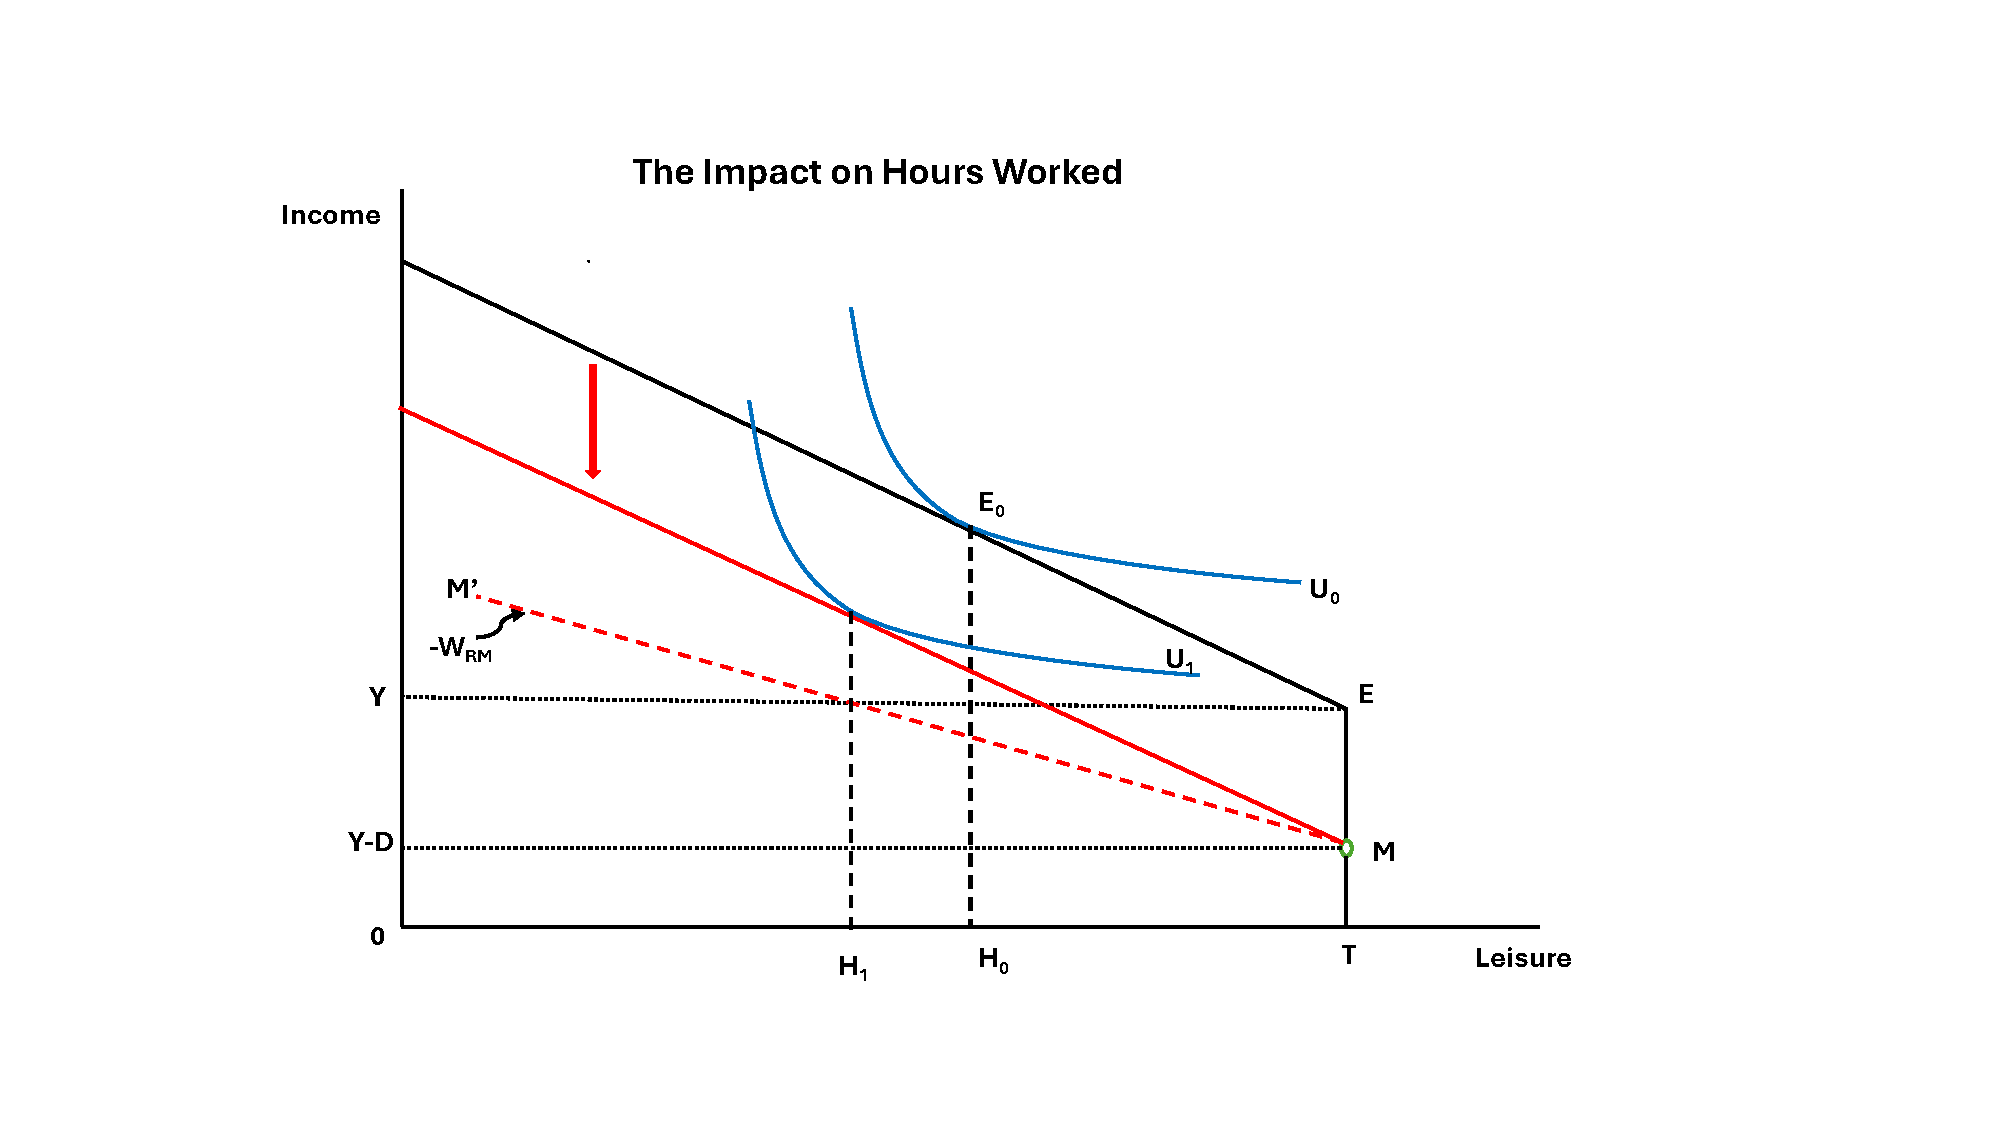
\includegraphics[scale=0.43]{Presentation4.pdf}
      %    \includegraphics[scale=.40]{one.pdf}
      \end{center}
  \end{figure}
\end{frame}

    \begin{frame}
  \frametitle{The effect of Child Care Costs on Labour Supply
}
\begin{figure}
    \begin{center}
      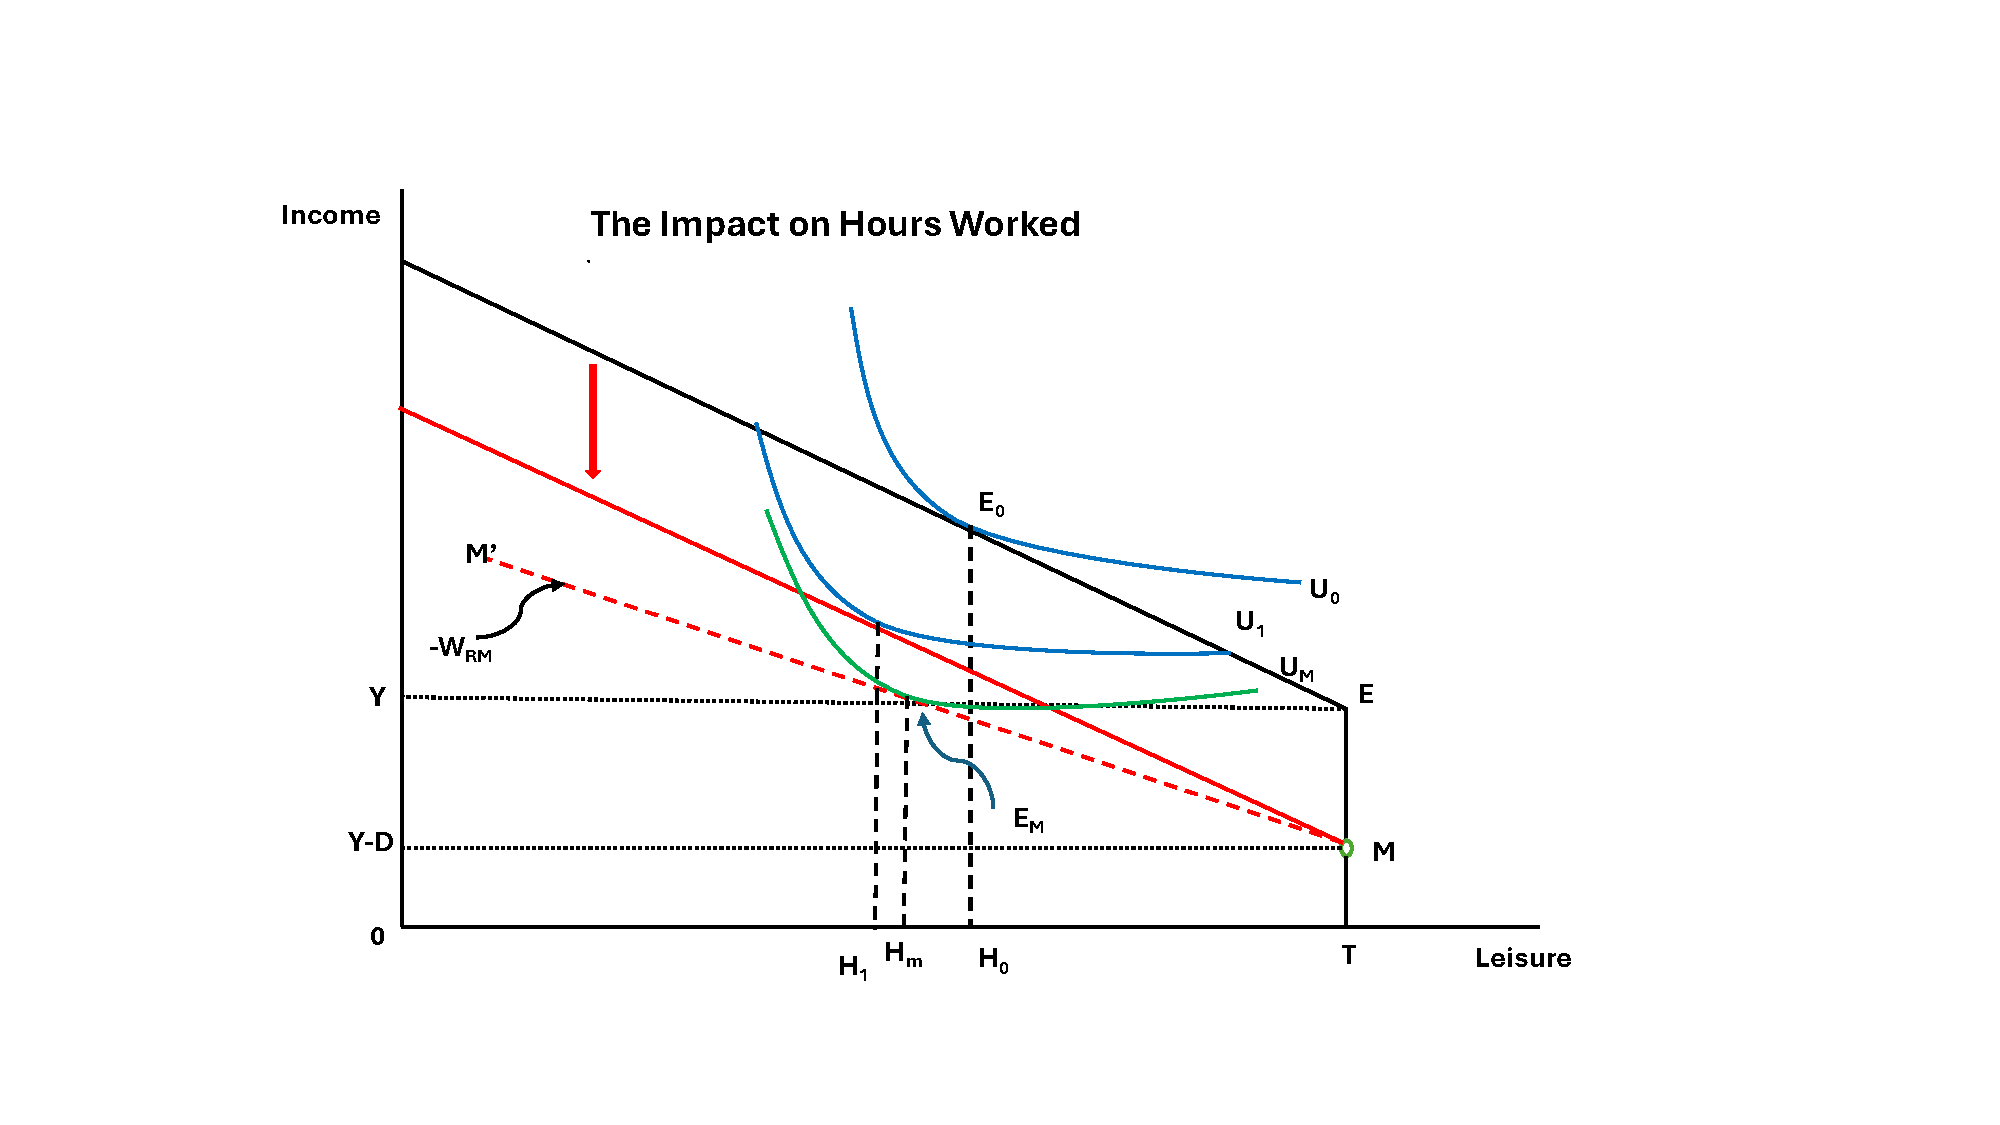
\includegraphics[scale=0.43]{Presentation5.pdf}
      %    \includegraphics[scale=.40]{one.pdf}
      \end{center}
  \end{figure}
\end{frame} 
 
 
 
 
 
 
   \begin{frame}
  \frametitle{The effect of Child Care Costs on Labour Supply
}
\begin{figure}
    \begin{center}
      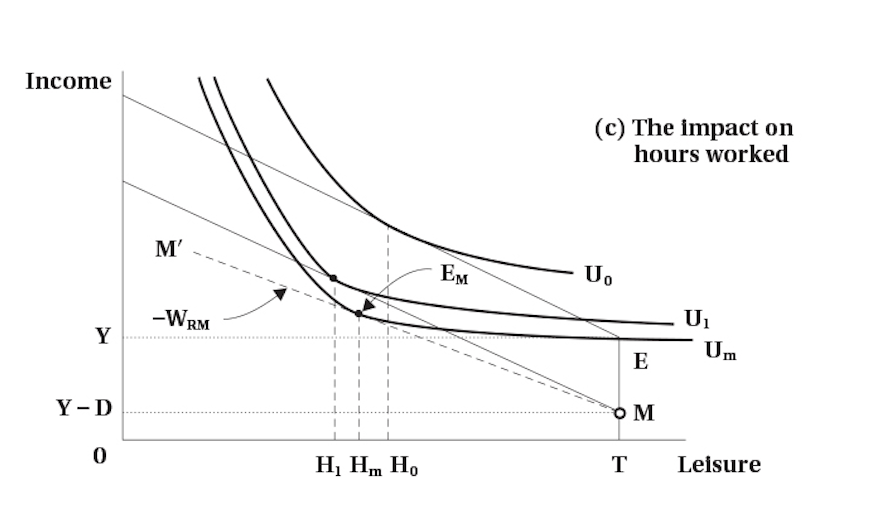
\includegraphics[scale=0.76]{CCB3.png}
      %    \includegraphics[scale=.40]{one.pdf}
      \end{center}
  \end{figure}
\end{frame}
 
 
    \begin{frame}
  \frametitle{The effect of Child Care Costs on Labour Supply}
\textbf{The impact on hours worked:}

\begin{itemize}

\item initial equilibrium:  at $E_{0}$ with hours of work $H_{0}$  and no child care costs
\item[]
\item the existence of fixed child care costs shifts the budget constraint down in a parallel fashion because market wages have not changed

\item[]
\item if leisure is a normal good - this pure income effect from the reduced income increases hours of work from $H_{0}$ to $H_{1}$ 
\item[]
\item when there are fixed costs, one has to work more hours to make up for the income loss associated with the costs of child care.

\end{itemize}

\end{frame}  
 
 
     \begin{frame}
  \frametitle{The effect of Child Care Costs on Labour Supply}



\textbf{Fixed child care costs also create a discontinuity or gap in the implied labour supply schedule}

\begin{itemize}
\item[]
\item the distance $TH_{m}$ indicates the number of hours below which it would not be worthwhile to enter the labour market - given the reservation wage $W_{RM}$ created by the child care costs EM

\item[]
\item it is not possible to amortize the fixed costs of entering the labour force over so few hours $\rightarrow$ there is a discrete jump in the labour supply from zero to $TH_{m}$ 
\item[]
\item geometrically,  it is not possible for there to be a tangency between the budget constraint MM' and the indifference curve $U_{M}$ in the region $E_{M}E$

\begin{itemize}
\item the slope of MM' is always greater than the slope of the indifference curve to the right $E_{M}$
\item in this way,  the child care costs discourage part-time work
\end{itemize}

\end{itemize}

\end{frame}  
 
 
 
  \begin{frame} \frametitle{Child Care Benefit}
\label{Child Care Benefit}

\begin{itemize}


\item Effects of child care costs

\begin{itemize}
\item Fixed child care costs increase reservation wage - decrease labour force participation

\item Fixed child care costs also affect hours-of-work
\begin{itemize}
\item Increased hours for those who participate
\item Create a discontinuity in labour supply -  making part-time work less likely
\item[]
\end{itemize}
\end{itemize}
\end{itemize}

Therefore,  child care benefit:
\begin{itemize}
\item encourages labour force participation and part-time work
\item[]
\item reduces the hours of work for those already participating
 \end{itemize}
 \end{frame}


\begin{frame}{Summary (1/2)}
\transfade
\begin{itemize}
  \item Income maintenance schemes top up low incomes from varied causes; some are better for transitory shocks, others for persistent low wages.
  \item The labour supply framework compares work incentives across designs via their budget constraints.
  \item \textbf{Demogrants:} Pure income effect; reduce work incentives at the margin.
  \item \textbf{Welfare:} Adverse incentives magnified by high clawbacks; policy levers include earnings disregards and lower implicit tax rates.
\end{itemize}
\end{frame}

\begin{frame}{Summary (2/2)}
\transfade
\begin{itemize}
  \item \textbf{NIT:} Smoother guarantee with partial clawback; still reduces work relative to no transfer.
  \item \textbf{Wage Subsidies/Refundable Credits:} Encourage work on phase-in but can reduce hours on flat/phase-out; participation effects often clearer.
  \item \textbf{UI/EI:} Insures transitory hours shocks; trade-off between search/matching and potential work disincentives.
  \item \textbf{Disability/Workers’ Comp:} Shift constraints and preferences; evaluate well-being across program designs.
  \item \textbf{Childcare:} Fixed costs affect participation margins; subsidies can raise LFPR, especially for parents.
\end{itemize}
\end{frame}

% ============================================================
\begin{frame}
\centering
\Huge{\textbf{Thank You!}} \\

\end{frame}

\end{document}
